% !TEX root = article.tex

\ifdefined\noauthorea
\begin{figure}[t]
\begin{center}
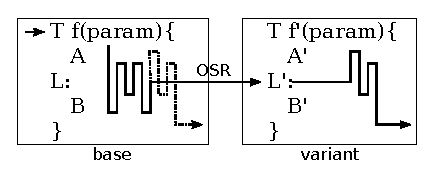
\includegraphics[width=0.6\columnwidth]{figures/overview-osr/overview-osr.eps}
\caption{\protect\label{fig:osr-dynamics} On-stack replacement dynamics: control is transferred via OSR from a point \textsf{L} of a base function \textsf{f} to a point \textsf{L'} in a variant \textsf{f'} of \textsf{f}.
  
  
  
  
  
  
  
  }
\end{center}
\end{figure}
\fi

\section{Overview}
\label{se:overview}

The key to platform independence in our work is to express the entire OSR machinery at intermediate code representation level, without resorting to machine-level code manipulation or special intrinsics of the intermediate language. %Before describing how this is achieved in LLVM, we provide an overview of our approach.

%\subsection{Overview}
%\label{ss:overview}

Consider the generic OSR scenario shown in \myfigure\ref{fi:osr-dynamics}. A base function \fbase\ is executed and it can either terminate normally (dashed lines), or an OSR event may transfer control to a variant \fvariant, which acts as a continuation function. The decision of whether an OSR should be fired at a given point \osrpoint\ of \fbase\ is based on an {\em OSR condition}. A typical example in JIT-based virtual machines is a profile counter reaching a certain hotness threshold, which indicates that \fbase\ is taking longer than expected and is worth optimizing. Another example is a guard testing whether \fbase\ has become unsafe and execution needs to fall back to a safe version \fvariant. This scenario includes deoptimization of functions generated with aggressive speculative optimizations. 

Several OSR implementations adjust the stack so that execution can continue in \fvariant\ with the current frame \cite{chambers1992design, suganuma2006region}. This requires manipulating the program state at machine code level and is highly ABI- and compiler-dependent. A simpler approach, which we follow in this article, consists of creating a new frame every time an OSR is fired, essentially regarding an OSR transition as a function call~\cite{Lameed_2013,webkit14}. 

Our implementation targets two general scenarios: 1) {\em resolved OSR}: \fvariant\ is known before executing \fbase\ as in the deoptimization example discussed above; 2) {\em open OSR}: \fvariant\ is generated when the OSR is fired, supporting deferred and profile-guided compilation strategies. In both cases, \fbase\ is instrumented before its execution to incorporate the OSR machinery. We call such OSR-instrumented version \fosrfrom.

\ifdefined\noauthorea
\begin{figure}[t]
\begin{center}
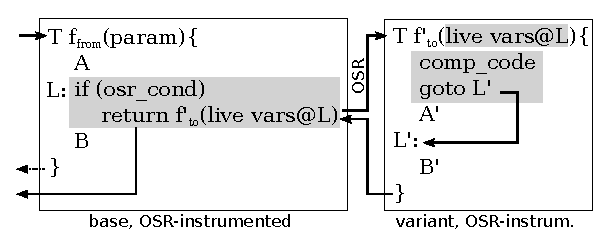
\includegraphics[width=0.7\columnwidth]{figures/overview-osr-final/overview-osr-final.eps}
\caption{\protect\label{fi:overview-osr-final} OSR-instrumented functions with resolved OSR call.}
\end{center}
\end{figure}
\fi

In the resolved OSR scenario (see \myfigure\ref{fi:overview-osr-final}), instrumentation consists of adding a check of the OSR condition and, if it is satisfied, a tail call that fires the OSR. The called function is an instrumented version of \fvariant, which we call \fosrto. The assumption is that \fosrto\ produces the same side-effects and return value that one would obtain by \fbase\ if no OSR was performed. Differently from \fvariant, \fosrto\ takes as input all live variables of \fbase\ at \osrpoint, executes an optional compensation code to fix the computation state ({\tt comp\_code}), and then jumps to a point \textsf{L'} from which execution can continue. The OSR practice often makes the conservative assumption that execution can always continue with the very same program state as the base function. However, this assumption may reduce the number of points where sound OSR transitions can be fired. Supporting compensation code in our framework adds flexibility, allowing OSR transitions to happen at arbitrary places in the base function.

\ifdefined\noauthorea
\begin{figure}[h!]
\begin{center}
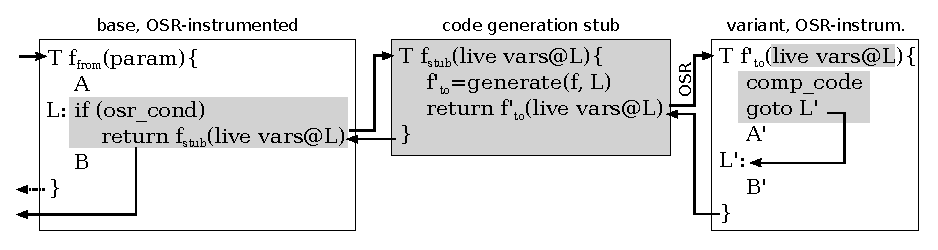
\includegraphics[width=1.0\columnwidth]{figures/overview-osr-open/overview-osr-open.eps}
\caption{\protect\label{fi:overview-osr-open} Functions of \ifauthorea{Figure~}{}\ref{fig:osr-dynamics} instrumented for open OSR.
  
  }
\end{center}
\end{figure}
\fi

The open OSR scenario is similar, with one main difference (see \myfigure\ref{fi:overview-osr-open}): instead of calling \fosrto\ directly, \fosrfrom\ calls a stub function \fstub, which first creates \fosrto\ and then calls it. Function \fosrto\ is generated by a function {\tt gen} that takes the base function \fbase\ and the OSR point \osrpoint\ as input. The reason for having a stub in the open OSR scenario, rather than directly instrumenting \fbase\ with the code generation machinery, is to minimize the extra code injected into \fbase. Indeed, instrumentation may interfere with optimizations, e.g., by increasing register pressure and altering code layout and instruction cache behavior.


\paragraph{Discussion.}
Instrumenting functions for OSR at a higher level than machine code yields several benefits: 
\begin{enumerate}
\item {\em Platform independence}: the OSR instrumentation code is lowered to native code by the compiler back-end, which handles the details of the target ABI; 
\item {\em Global optimizations}: lowering OSR instrumentation code along with the application code can generate faster code than local binary instrumentation. For instance, dead code elimination can suppress from \fosrto\ portions of code that would no longer be needed when jumping to the landing pad \textsf{L'}, producing smaller code and enabling better register allocation and instruction scheduling.
\item {\em Debugging and Profiling}: preserving ABI conventions in the native code versions of \fosrfrom, \fstub, and \fosrto\ helps debuggers and profilers to more precisely locate the current execution context and collect more informative data.
%avoiding low-lever tampering with stack frames can more easily preserve ABI calling conventions
\item {\em Abstraction}: being entirely encoded using high-level language constructs (assignments, conditionals, function calls), the approach is amenable to a clean instrumentation API that abstracts the OSR implementation details, allowing a front-end to focus on where to insert OSR points independently of the final target architecture.
%by analyzing code at an intermediate representation level.
\end{enumerate}

\noindent A natural question is whether encoding OSR at a higher level of abstraction can result in poorer performance than binary code approaches. We address this issue in \mysection\ref{se:osr-llvm}, where we analyze the OSR machine code generated for an x86-64 target, and in \mysection\ref{se:experiments}, where OSR performance is measured on classical benchmarks.